\chapter{Design}
	For reasons of clarity, the description of the design of the software follows a top-down approach. The first section gives an overview of the software and the others study in deep specific aspects of it.

	To better explain the contents and the structure of the design, the description is supported by \mbox{UML} diagrams. As the following sections describe the software at difference levels of detail, the diagrams reflect this approach. In the first section, for example, the diagram is used only to present the classes in the overall structure. For this reason it contains only the names of the classes. Further details are added in the diagrams in the next sections, according with the top-down approach of the chapter.

	\section{Overview of the design}
	The software is composed of four main parts, one for processing images and videos, one for containing the hierarchy of the objects recognized during such processing, one for allowing ACT-R to communicate with the software and one containing all the utility functions used by all the other parts.

	\begin{figure}[h]
	  \begin{center} 
	    \fbox{	
	       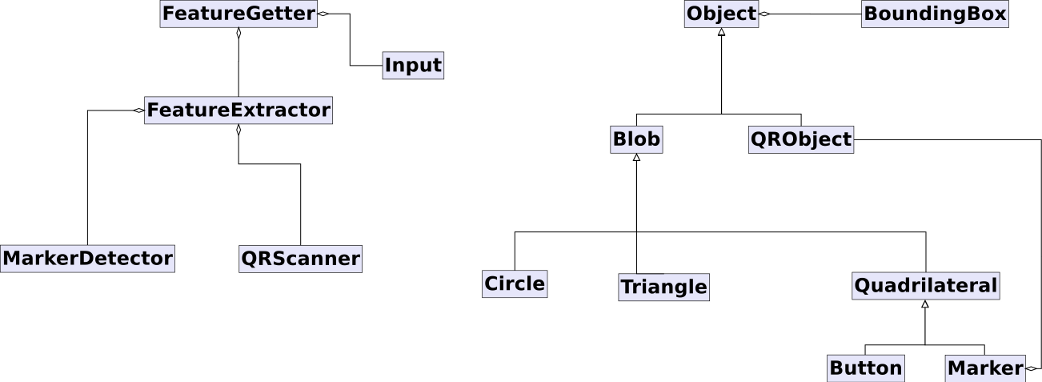
\includegraphics[scale=0.55]{images/ch_05/progettazione_overview2.png}
	    }
	  \end{center} 
	  \caption{\textit{Class diagram illustrating a high level overview of the design of the software }}  
	  \label{fig:swArchitecture}
 	\end{figure}		

	Image \ref{fig:swArchitecture} shows a class diagram which describes two of the parts that compose the software. 
	The part dedicated to the processing of images and video is located on the left and is composed by the classes \emph{Proxy}, \emph{FeatureGetter}, \emph{FeatureExtractor}, \emph{Input}, \emph{MarkerDetector} and \emph{QRScanner}.
	The object hierarchy, which is shown on the right, contains the classes \emph{Object}, \emph{BoundingBox}, \emph{Blob}, \emph{QRObject}, \emph{Circle}, \emph{Triangle}, \emph{Quadrilateral}, \emph{Button} and \emph{Marker}.

	

	The other two parts are not included in the design diagrams for different reasons. 
	According with the non-functional requirements, the team planned to try different solutions in order to implement the communication between the software and ACT-R. As different approaches can lead to different architectures, this part has not been designed a priori.
	Regarding the utility part, as it depends strongly by the implementations choices, it is very instable and volatile. Moreover, it is heavily influenced by the chosen communication technique, which, as just described, has not been planned.
	For these reasons, according to the agile development the team decided not to spend time in planning a fixed structure for it.
	
	
	\section{Feature Extractors}	
	
	

\begin{comment} 
	\section{Class Hierarchy}
	
	\section{Communication with ACT-R}

  
  \section{The Whole Software}
  The aim of the 
  \begin{figure}[h]
	  \begin{center} 
		%TODO: aggiungere immagine	
	    %\includegraphics[scale=0.1]{images/ch_04/classDesign.jpg}
	  \end{center} 
	  \caption{\textit{Class diagram of the whole software }}  
	  \label{fig:swArchitecture}
  \end{figure}
  \todo{cambiare l immagine e aggiungere la descrizione...}.

  
  \section{The Class Hierarchy}
  \begin{figure}[h]
	  \begin{center} 
		%TODO: aggiungere immagine
	    %\includegraphics[scale=0.2]{images/ch_04/designClassObjectHierarchy.jpeg}
	  \end{center} 
	  \caption{\textit{Class hierarchy of the recognized objects}}  
	  \label{fig:callHierarchy}
  \end{figure}
   {\newpage}
   {\newpage}
   {\newpage}
   {\newpage}
  The picture above describes the hierarchy of the classes defined to contain the objects detected in the images. The \textit{Object} class represents a generic object that can be found in an image. Thus, everything which is different from the background can be seen as an instance of the \textit{Object} class. Every object must be bounded by a \textit{bounding box}. This structure is represented by the \textit{BoundingBox} class. All the bounding boxes have rectangular shape. The requirements were such that it was not necessary to define more complicate shapes \todo{migliorare questa frase, fa schifo}. The \textit{attended} attribute of the \textit{Object}  class is set to \textit{true} if the object has been already returned to ACT-R, otherwise it is set to \textit{false}. The \textit{rotation} is a value that gives the amount of the rotation in the counterclockwise directions starting from the horizontal direction \todo{controllare la correttezza}. \todo{vedere se il metodo getChunk esiste ancora}\todo{se 
non esiste eliminarlo 
dall immagine}.
  Besides the generic objects, there are two categories of object that can be found in the processed images, the \textit{QR codes} and the \textit{simples shapes}. A simple shape can be, for example, a circle, a square, a rectangle or a triangle. The QR codes is represented in the hierarchy with the \textit{QRObject} class, the generic shape with the \textit{Blob} class.
  This class has the \textit{area} parameter, which stands for the area of the object in pixel, and the  \textit{getArea} method, which returns this value. The \textit{Blob} class is realized by three classes, \textit{Circle}, \textit{Triangle} and \textit{Quadrilateral}. 
  The first one has, as parameters, the \textit{center} and the \textit{radius} of the circle itself.
  The parameters of the \textit{Triangle} and the \textit{Quadrilateral} classes are respectively three and four points, which represent the vertices of the shape. Notice that the \textit{Quadrilateral} class defines every polygon with four sides and four vertices. Thus, rectangles and squares can be instances of this class. 
  The \textit{Button} class is a realization of the \textit{Quadrilateral} class. This is because, as a requirement, buttons have always rectangular or squared shapes. The additional information they add is the \textit{text}, that is a simple message that is always present in a button. It is represented by the \textit{text} attribute. 
  The \textit{Point} class identifies a generic point in the bidimensional space. Its parameters, \textit{x} and \textit{y}, are the two coordinates in the plane.
 
  \todo{... aggiungere, correggere o finire}

  
 \end{comment} 
  
  
  
